As described in Section.~\ref{sec:4.2}, JES and JER systematic uncertainties are considered for the String resonances. In this study, three NPs from the JES and 7 NPs from the JER are studied on the normalised template shapes. 

The impact from JES on the signal template is evaluated by comparing the nominal distribution to the distribution from each JES NP. The impact from JER on the signal template is evaluated by considering the shift in the RMS (or standard deviation) of the distribution from each JER NP. Such signal shits are parameterised by using a Gaussian function fit to the most significant bins around
the maximum mean value of the distribution. 


Figure~\ref{fig2} shows an example for the $\Ms = 8$~TeV signal sample
and the JES GroupedNP\_3 group.
This represents the histogram of one of the systematics that are used in
the limit calculation.
The GroupedNP\_3 group was found to give the biggest shift in the signal
mean.

For the signal samples at all masses and widths, the reconstructed peak of signal is shifted low relative to the generated peak by $\sim
0.92\Ms$, even before taking the JES or JER systematic
uncertainties into account.

\begin{figure}[htb]
\begin{center}
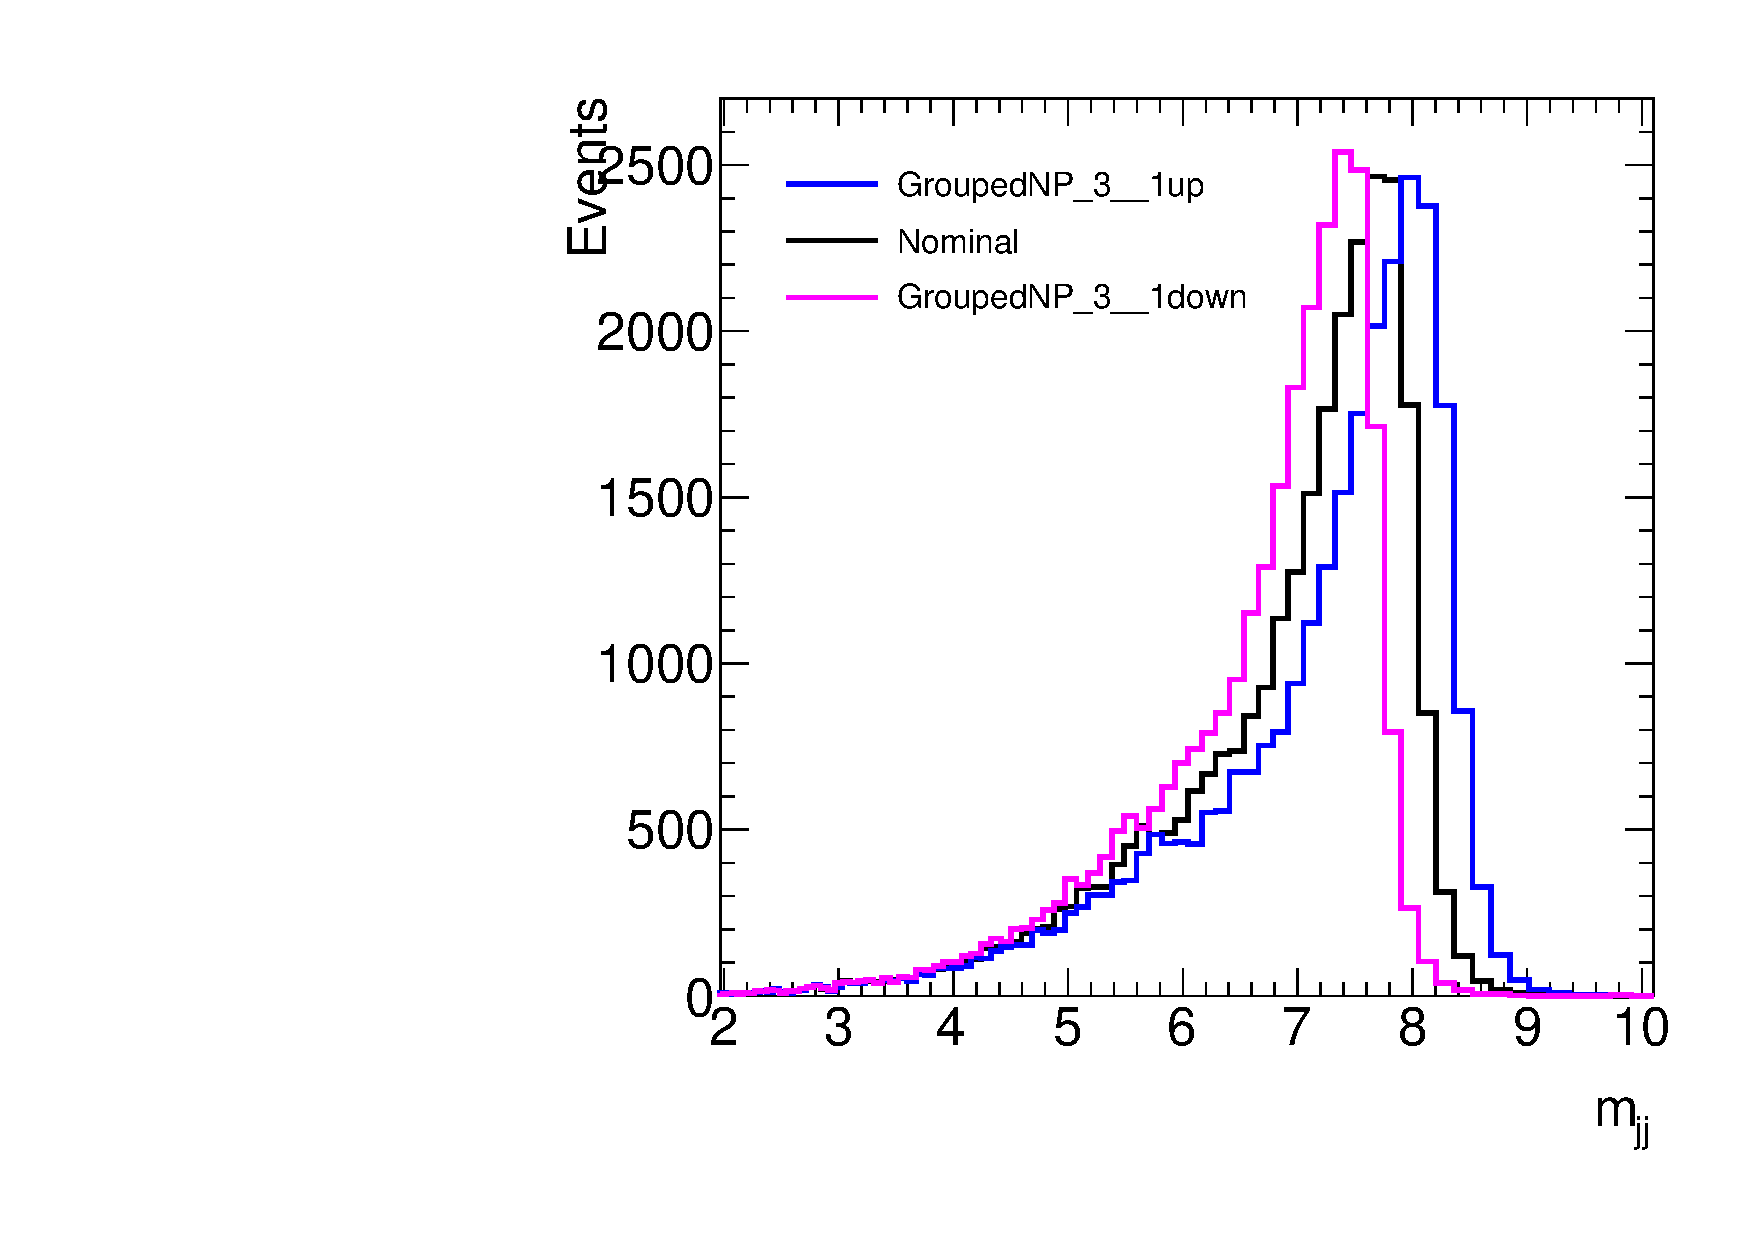
\includegraphics[width=0.65\linewidth]{fig/strings/JES_shift}
\end{center}
\caption{\mjj\ distribution for the $\Ms = 8$~TeV string sample (nominal).
Also shown are the distributions using the jet energy scale
GroupedNP\_3 one standard deviation up and down systematic uncertainties.}
\label{fig2}
\end{figure}

Figure~\ref{fig3} shows the relative shift in the mean of the \mjj\
distribution due to the JES uncertainty and the relative change in RMS
of the \mjj\ distribution due to the JER uncertainty. 
Although all the NPs are applied independently in the
limit calculations, here only shows all three JES mean shifts in quadrature
and all seven JER resolutions differences in quadrature. 

\begin{figure}[htb]
\begin{center}
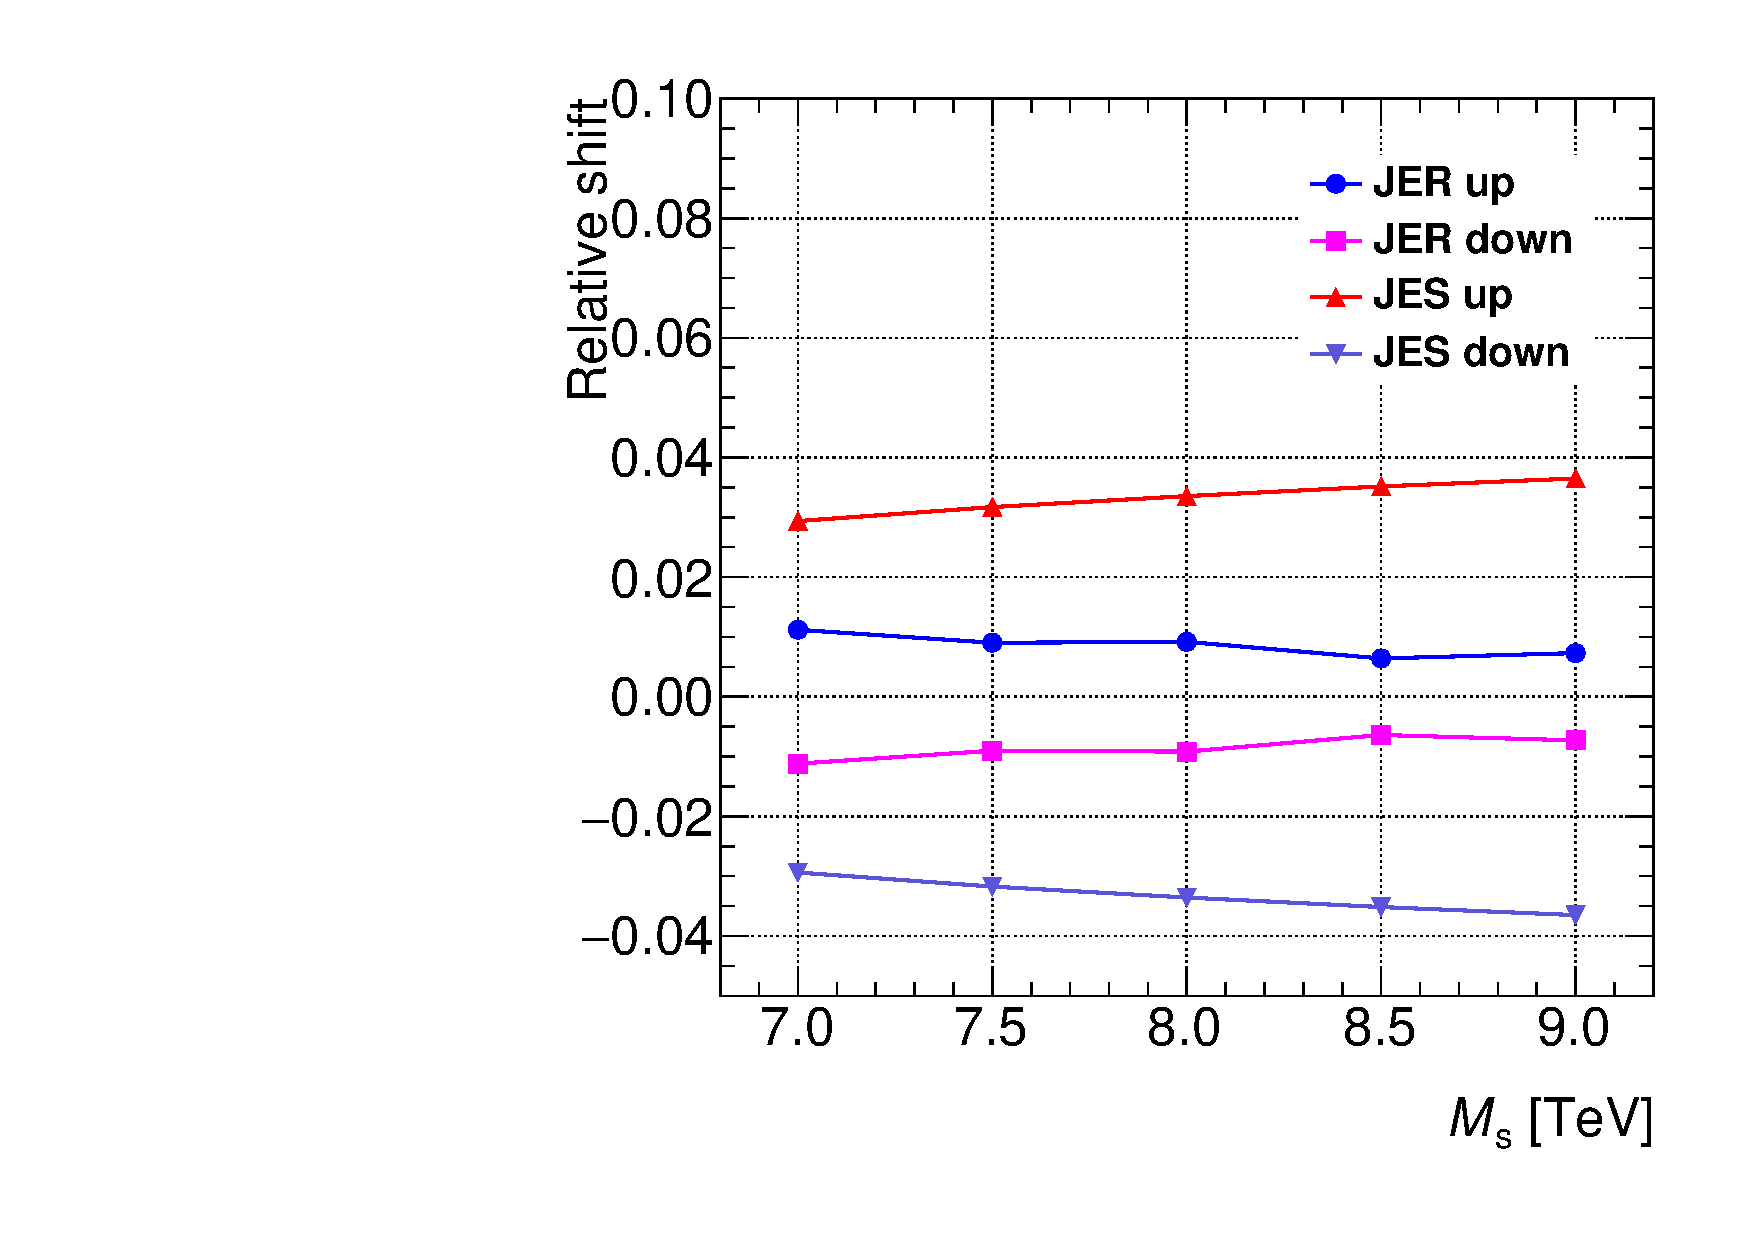
\includegraphics[width=0.65\linewidth]{fig/strings/JES_JER}
\end{center}
\caption{Relative shift in the mean of the \mjj\ distributions for each
string sample due to jet energy scale uncertainty, and relative change
in the RMS of the \mjj\ distributions for each string sample due to the
jet energy resolution uncertainty.
The changes due to each nuisance parameter group are added in
quadrature.}
\label{fig3}
\end{figure}

The changes in signal acceptance after applied JES and JER uncertainties are
added in quadrature and determined to be less than 0.06\%.  Such small uncertainty can be ignored for the signal
acceptance.


The changes in mean of the signal distributions after applied the JES uncertainty is dominated by GroupedNP\_3 and less than 4\%. The change in RMS of the signal distributions after applied the JER uncertainty
is less than 1.2\%. This is the most significant uncertainty for the lowest \Ms signal sample and
each of the seven values that are added in quadrature do not have a
dominate component.


\FloatBarrier